\documentclass[ignorenonframetext]{beamer}
\usetheme{sts}
\title[HW-7-2]{Homework Sheet 7, Ex. 2}

\author{Büchler P., Lohmann N.J}
\institute{Institute for Software Systems}
\date{\today}

\begin{document}

\begin{document}
\newcommand{\slide1}{%
\begin{frame}<presentation>[plain]
\titlepage{}
\end{frame}
}


\newcommand{\slide2}{
\begin{frame}<presentation>
\frametitle{Contents}
%\tableofcontents[hideallsubsections]{}
\tableofcontents[]{}
\end{frame}
}

\section{Ex.2}
\subsection{Data Flow}


\begin{frame}{Data Flow Graph}
\begin{figure}[h]    
\centering
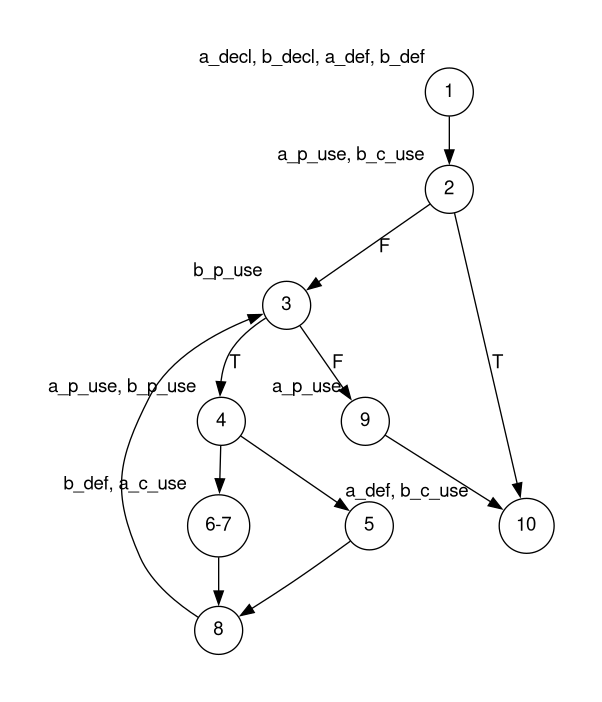
\includegraphics[scale=0.3]{dataflowgraph.png}
\end{figure}
\end{frame}

\begin{frame}


\frametitle{DU-Paths (a)}
\begin{itemize}
\item 1-2, 1-2-3-9
\item 1-2-3-4, 1-2-3-4-6-7, 1-2-3-4-6-7-9
\item 5-8-3-4,  5-8-3-4-6-7 
\item 5-8-3-9
\end{itemize}
\end{frame}

\begin{frame}
\frametitle{DU-Paths (b)}
\begin{itemize}
\item 1-2, 1-2-3
\item 1-2-3-4, 1-2-3-4-5
\item 6-7-8-3, 6-7-8-3-4, 6-7-8-3-4-5 
\end{itemize}
\end{frame}

\subsection{Test Suite}

\begin{frame}{Test Suite}
\begin{tabular}{c c}
Test      & \#1          \\
Test Path & 1-2          \\
Coverage  & 1-2          \\
Input     & a = 0, b = 0 \\
Output    & 0             
\end{tabular}
\newline
\begin{tabular}{c c}
Test      & \#2          \\
Test Path & 1-2-3-9          \\
Coverage  & 1-2, 1-2-3-9          \\
Input     & a = 1, b = 0 \\
Output    & 1             
\end{tabular}
\end{frame}

\begin{frame}{Test Suite cont.}
\begin{tabular}{c c}
Test      & \#3          \\
Test Path & 1-2-3-4-6-7-8-3-9          \\
Coverage  & 1-2, 1-2-3-4, 1-2-3-4-6-7, 1-2-3-4-6-7-8-9          \\
Input     & a = 1, b = 1 \\
Output    & 1             
\end{tabular}
\begin{tabular}{c c}
Test      & \#4          \\
Test Path & 1-2-3-4-5-8-3-4-6-7-8-3-9          \\
Coverage  & 1-2, 1-2-3-4, 5-8-3-4, 5-8-3-4-6-7, 5-8-3-4-9         \\
Input     & a = 2, b = 1 \\
Output    & 1             
\end{tabular}
\end{frame}


\subsection{Comparison}
\begin{frame}{Comparison Data Flow vs. Branch coverage}
    For 100\% multiple-condition coverage, \(c = 3 \implies 2^c = 8\)
    \newline
    Twice the No. of Data-Flow cases, due to test cases of the form \(a = 0, b = * \).
    Which never go further than the path 1-2-3-9.
\end{frame}

\begin{frame}{Thanks}
    \center 
    Thank you for your attention!
\end{frame}

\end{document}
